\documentclass[journal,12pt,twocolumn]{IEEEtran}
%
\usepackage{setspace}
\usepackage{gensymb}
%\doublespacing
\singlespacing

\usepackage[cmex10]{amsmath}
\usepackage{amsthm}
%\usepackage{iithtlc}
\usepackage{mathrsfs}
\usepackage{txfonts}
\usepackage{stfloats}
\usepackage{bm}
\usepackage{cite}
\usepackage{cases}
\usepackage{subfig}
%\usepackage{xtab}
\usepackage{longtable}
\usepackage{multirow}
%\usepackage{algorithm}
%\usepackage{algpseudocode}
\usepackage{enumitem}
\usepackage{mathtools}
\usepackage{steinmetz}
\usepackage{tikz}
\usepackage{circuitikz}
\usepackage{verbatim}
\usepackage{tfrupee}
\usepackage[breaklinks=true]{hyperref}
%\usepackage{stmaryrd}
\usepackage{tkz-euclide} % loads  TikZ and tkz-base
%\usetkzobj{all}
\usetikzlibrary{calc,math}
\usepackage{listings}
    \usepackage{color}                                            %%
    \usepackage{array}                                            %%
    \usepackage{longtable}                                        %%
    \usepackage{calc}                                             %%
    \usepackage{multirow}                                         %%
    \usepackage{hhline}                                           %%
    \usepackage{ifthen}                                           %%
  %optionally (for landscape tables embedded in another document): %%
    \usepackage{lscape}     
\usepackage{multicol}
\usepackage{chngcntr}
%\usepackage{enumerate}

%\usepackage{wasysym}
%\newcounter{MYtempeqncnt}
\DeclareMathOperator*{\Res}{Res}
%\renewcommand{\baselinestretch}{2}
\renewcommand\thesection{\arabic{section}}
\renewcommand\thesubsection{\thesection.\arabic{subsection}}
\renewcommand\thesubsubsection{\thesubsection.\arabic{subsubsection}}

\renewcommand\thesectiondis{\arabic{section}}
\renewcommand\thesubsectiondis{\thesectiondis.\arabic{subsection}}
\renewcommand\thesubsubsectiondis{\thesubsectiondis.\arabic{subsubsection}}

% correct bad hyphenation here
\hyphenation{op-tical net-works semi-conduc-tor}
\def\inputGnumericTable{}                                 %%

\lstset{
%language=C,
frame=single, 
breaklines=true,
columns=fullflexible
}
\newenvironment{amatrix}[1]{%
  \left(\begin{array}{@{}*{#1}{c}|c@{}}
}{%
  \end{array}\right)
}
\DeclarePairedDelimiter\abs{\lvert}{\rvert}%
\DeclarePairedDelimiter\norm{\lVert}{\rVert}%

% Swap the definition of \abs* and \norm*, so that \abs
% and \norm resizes the size of the brackets, and the 
% starred version does not.
\makeatletter
\let\oldabs\abs
\def\abs{\@ifstar{\oldabs}{\oldabs*}}
%
\let\oldnorm\norm
\def\norm{\@ifstar{\oldnorm}{\oldnorm*}}
\makeatother

\newtheorem{theorem}{Theorem}[section]
\newtheorem{problem}{Problem}
\newtheorem{proposition}{Proposition}[section]
\newtheorem{lemma}{Lemma}[section]
\newtheorem{corollary}[theorem]{Corollary}
\newtheorem{example}{Example}[section]
\newtheorem{definition}[problem]{Definition}
%\newtheorem{thm}{Theorem}[section] 
%\newtheorem{defn}[thm]{Definition}
%\newtheorem{algorithm}{Algorithm}[section]
%\newtheorem{cor}{Corollary}
\newcommand{\BEQA}{\begin{eqnarray}}
\newcommand{\EEQA}{\end{eqnarray}}
\newcommand{\define}{\stackrel{\triangle}{=}}
\bibliographystyle{IEEEtran}
%\bibliographystyle{ieeetr}
\providecommand{\mbf}{\mathbf}
\providecommand{\pr}[1]{\ensuremath{\Pr\left(#1\right)}}
\providecommand{\qfunc}[1]{\ensuremath{Q\left(#1\right)}}
\providecommand{\sbrak}[1]{\ensuremath{{}\left[#1\right]}}
\providecommand{\lsbrak}[1]{\ensuremath{{}\left[#1\right.}}
\providecommand{\rsbrak}[1]{\ensuremath{{}\left.#1\right]}}
\providecommand{\brak}[1]{\ensuremath{\left(#1\right)}}
\providecommand{\lbrak}[1]{\ensuremath{\left(#1\right.}}
\providecommand{\rbrak}[1]{\ensuremath{\left.#1\right)}}
\providecommand{\cbrak}[1]{\ensuremath{\left\{#1\right\}}}
\providecommand{\lcbrak}[1]{\ensuremath{\left\{#1\right.}}
\providecommand{\rcbrak}[1]{\ensuremath{\left.#1\right\}}}

\providecommand{\system}{\overset{\mathcal{H}}{ \longleftrightarrow}}
	%\newcommand{\solution}[2]{\textbf{Solution:}{#1}}
\newcommand{\solution}{\noindent \textbf{Solution: }}
\newcommand{\cosec}{\,\text{cosec}\,}
\providecommand{\dec}[2]{\ensuremath{\overset{#1}{\underset{#2}{\gtrless}}}}
\newcommand{\myvec}[1]{\ensuremath{\begin{pmatrix}#1\end{pmatrix}}}
\newcommand{\mydet}[1]{\ensuremath{\begin{vmatrix}#1\end{vmatrix}}}
%\numberwithin{equation}{section}
\numberwithin{equation}{subsection}
%\numberwithin{problem}{section}
%\numberwithin{definition}{section}
\makeatletter
\@addtoreset{figure}{problem}
\makeatother
\let\StandardTheFigure\thefigure
\let\vec\mathbf
\usepackage{mathtools, nccmath}

\begin{document}

\begin{center}
\huge Assignment 6\\

\large Shaik Zeeshan Ali\\
\large AI20MTECH11001\\
\end{center}
\begin{abstract}
This document is about tracing a parabola
\end{abstract}
Download all python codes from 
\begin{lstlisting}
https://github.com/Zeeshan-IITH/IITH-EE5609/new/master/codes
\end{lstlisting}

and latex-tikz codes from 
\begin{lstlisting}
https://github.com/Zeeshan-IITH/IITH-EE5609
\end{lstlisting}
\section{problem}
Trace the following parabola
\begin{align}
    4x^2-4xy+y^2-12x+6y+9=0
\end{align}
\section{construction}
The given quadratic equation can be written in the matrix form as
\begin{align}
    \vec{x}^T\myvec{4&-2\\-2&1}\vec{x}+2\myvec{-6&3}\vec{x}+9=0\label{eq:1}
\end{align}
Calculating the parameters
\begin{align}
    \mydet{\vec{V}}=\mydet{4&-2\\-2&1}=0\\
    \mydet{\vec{V}&\vec{u}\\\vec{u}^T&f}=\mydet{4&-2&-6\\-2&1&3\\-6&3&9}=0
\end{align}
Therefore the given parabola equation is a degenerate.\par
The characteristic equation of $\vec{V}$ will be
\begin{align}
    \mydet{\vec{V}-\lambda\vec{I}}&=\mydet{4-\lambda&-2\\-2&1-\lambda}\\
    &=\lambda^2-5\lambda\\
    &\lambda_1=0,\lambda_2=5
\end{align}
The eigen vectors are the nullspace of the matrix $\vec{V}-\lambda\vec{I}$.For $\lambda_1=0$
\begin{align}
    \myvec{4&-2\\-2&1}\xleftrightarrow{R_2=2R_2+R_1}\myvec{4&-2\\0&0}\\
    p_1=\myvec{1\\2}
\end{align}
Therefore the normalized eigen vector will be
\begin{align}
    p_1=\myvec{\frac{1}{\sqrt{5}}\\\frac{2}{\sqrt{5}}}
\end{align}
For $\lambda_2=5$
\begin{align}
    \myvec{-1&-2\\-2&-4}\xleftrightarrow{R_2=R_2-2R_1}\myvec{-1&-2\\0&0}\\
    p_2=\myvec{-2\\1}
\end{align}
Therefore the normalized eigen vector will be
\begin{align}
    p_2=\myvec{-\frac{2}{\sqrt{5}}\\\frac{1}{\sqrt{5}}}
\end{align}
Therefore the transformation matrix will be
\begin{align}
    \vec{P}=\myvec{p_1&p_2}=\myvec{\frac{1}{\sqrt{5}}&-\frac{2}{\sqrt{5}}\\\frac{2}{\sqrt{5}}&\frac{1}{\sqrt{5}}}
\end{align}
The value of $\eta$ will be
\begin{align}
    \eta&=2p_1^T\vec{u}\\
    &=2\myvec{\frac{1}{\sqrt{5}}&\frac{2}{\sqrt{5}}}\myvec{-6\\3}\\
    &=0
\end{align}
\section{Equation of the coincident line}
The vertex of the degenerate hyperbola can be calculated as
\begin{align}
    \myvec{\vec{u}^T+\frac{\eta}{2}p_1^T\\\vec{V}}c=\myvec{-f\\\frac{\eta}{2}p_1-\vec{u}}\\
    \myvec{-6&3\\4&-2\\-2&1}c=\myvec{-9\\6\\-3}\\
    \myvec{-6&3&-9\\4&-2&6\\-2&1&-3}\xleftrightarrow{R_3=3R_3-R_1}\myvec{-6&3&-9\\4&-2&6\\0&0&0}\\
    \myvec{-6&3&-9\\4&-2&6\\0&0&0}\xleftrightarrow{R_2=\frac{3}{2}R_2+R_1}\myvec{-6&3&-9\\0&0&0\\0&0&0}
\end{align}
Therefore the vertex is $c=\myvec{1\\-1}$ is one of the solution.\par
Applying affine transformation on equation \eqref{eq:1},we get
\begin{align}
    \vec{y}^T\vec{D}\vec{y}=0\\
    \vec{y}^T\myvec{0&0\\0&5}\vec{y}=0\\
    5y^2=0\\
    y^2=0
\end{align}
So the line is $y=0$.\par
Applying inverse affine tranformation on the line we get
\begin{align}
    \myvec{0&1}\vec{P}^{-1}\brak{\vec{x}-c}=0\\
    \myvec{0&1}\myvec{\frac{1}{\sqrt{5}}&\frac{2}{\sqrt{5}}\\-\frac{2}{\sqrt{5}}&\frac{1}{\sqrt{5}}}\vec{x}-\myvec{0&1}\myvec{\frac{1}{\sqrt{5}}&\frac{2}{\sqrt{5}}\\-\frac{2}{\sqrt{5}}&\frac{1}{\sqrt{5}}}\myvec{1\\-1}=0\\
    \myvec{-\frac{2}{\sqrt{5}}&\frac{1}{\sqrt{5}}}\vec{x}+\frac{3}{\sqrt{5}}=0\\
    -\frac{2x}{\sqrt{5}}+\frac{y}{\sqrt{5}}+\frac{3}{\sqrt{5}}\\
    2x-y-3=0
\end{align}
Therefore the equation of coincident lines is $\brak{2x-y-3}^2=0$.
\begin{figure}[t]
    \centering
    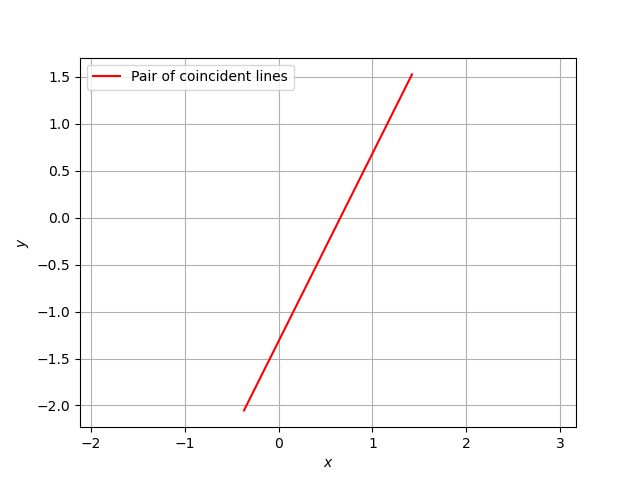
\includegraphics[width=\columnwidth]{Fig_a6.png}
    \caption{Pair of coincident lines}
    \label{fig:my_label}
\end{figure}
\end{document}
